% !TEX root=../MA119-Main.tex


\begin{tcolorbox}[colback=white,colframe=cyan, title filled=false, coltitle=cyan, enhanced, attach boxed title to top center={yshift=-3mm,yshifttext=-1mm}, fonttitle=\bfseries, boxed title style={size=small,colback=white},
title=Exponential  function
]
Let $b$ be a positive number other than $1$, i.e. $b>0$ and $b\neq 1$, the exponential function $f$ of $x$ with the base $b$ is defined as
\[f(x)=b^x\quad\quad\text{or}\quad\quad y=b^x.\]

Graphs of exponential functions:
\begin{center}
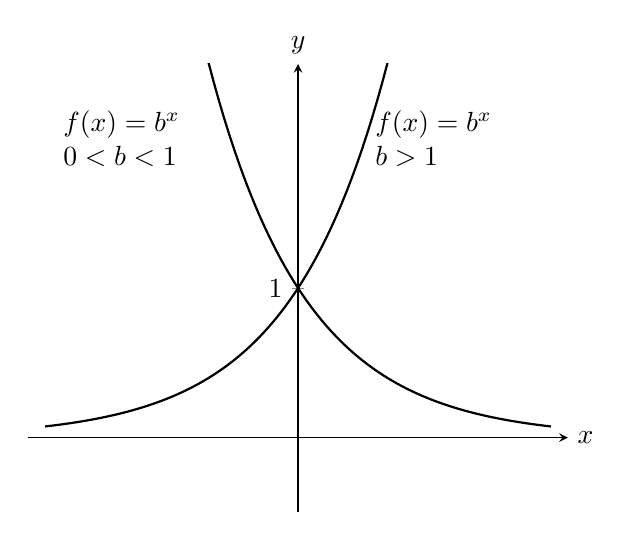
\begin{tikzpicture}
 \begin{axis}[%grid=both, 
 ymin=-0.5,ymax=2.5,xmax=4,xmin=-4, xtick=\empty,ytick=\empty, extra y ticks={1}, 
 axis lines = middle,xlabel=$x$,ylabel=$y$, 
x label style={anchor=west}, y label style={anchor=south}, 
%label style ={at={(ticklabel cs:1.1)}, font={\tiny}}
]
 \addplot[thick, samples=100, domain=-3.75:3.75]   {2^x};
 \addplot[thick, samples=100, domain=-3.75:3.75]   {(1/2)^x};           
\node[anchor=east] at (axis cs:-1,2)   {\parbox{2cm}{$f(x)=b^x$\\ $0< b<1$}};   
\node[anchor=west] at (axis cs:1,2)   {\parbox{2cm}{$f(x)=b^x$\\ $b>1$}};           
  \end{axis}
\end{tikzpicture}
\end{center}
 
\end{tcolorbox}

\begin{tcolorbox}[colback=white,colframe=cyan, title filled=false, coltitle=cyan, enhanced, attach boxed title to top center={yshift=-3mm,yshifttext=-1mm}, fonttitle=\bfseries, boxed title style={size=small,colback=white},
title=The natural number $e$
]
The natural number $e$ is the number that the expression $\left(1+\dfrac1n\right)^n$ approaches to as $n$ takes on increasingly large values. 
Approximately,  $e\approx2.718281827$.
\end{tcolorbox}


\begin{tcolorbox}[colback=white,colframe=cyan, title filled=false, coltitle=cyan, enhanced, attach boxed title to top center={yshift=-3mm,yshifttext=-1mm}, fonttitle=\bfseries, boxed title style={size=small,colback=white},
title=Compound interest
]
After $t$ years, the balance, $A$ in an account with a principal $P$ and annual interest rate $r$ is given by the following formulas:
 
\begin{enumerate}
\item For $n$ compounding periods per year: $A=P\left(1+\dfrac{r}{n}\right)^{nt}$.
\item For compounding continuously: $A=Pe^{rt}$.
\end{enumerate}
\end{tcolorbox}


\begin{exercise}
The exponential function $f(x)=42.2(1.56)^x$ models the average amount spent, $f(x)$, in dollars, at a shoping mall after $x$ hours. What is the average amount spent, to the nearest dollar, after three hours.
\end{exercise}

\iffalse
\begin{exercise}
A car is depreciating according the formula: $V=25000(3.2)^{-0.05x}$ where $x$ is the age of the car in years. Find the value of the car when it is five years old. 
\end{exercise}
\fi


\begin{exercise}
A sum of \$10,000 is invested at an annual rate of 8\%, Find the balance in the account after 5 years subject to 
\begin{enumerate}
\item quarterly compounding,
\item continuous compounding.
\end{enumerate}
\end{exercise}


\iffalse
\begin{exercise}
A sum of \$20,000 is invested at an annual rate of 5.5\%, Find the balance in the account after 5 years subject to 
\begin{enumerate}
\item mothly compounding,
\item continuous compounding.
\end{enumerate}
\end{exercise}
\fi


\begin{exercise}[Optional]
Sketch the graph of each function and find its range.\\

\noindent
\begin{enumerate*}[label=\arabic*)~~]
\item $f(x)=3^x$\hspace{0.3\textwidth}
\item $f(x)=(\frac13)^x$
\end{enumerate*}

\noindent
\begin{minipage}{\textwidth}
\begin{minipage}{0.5\textwidth}
\begin{center}
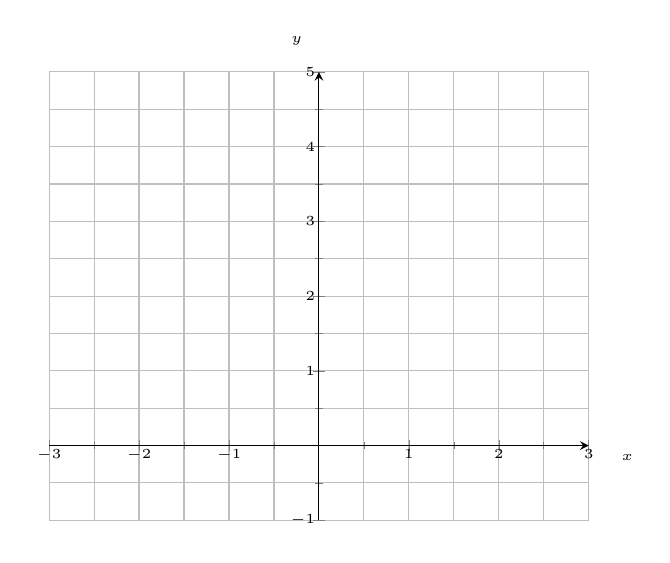
\begin{tikzpicture}
 \begin{axis}[grid=both, ymin=-1,ymax=5,xmax=3,xmin=-3,xtick={-3,-2,...,3},ytick={-1,0,...,5},minor tick num=1, axis lines = middle,xlabel=$x$,ylabel=$y$, 
x tick label style={yshift=1ex,font={\tiny}}, y tick label style={xshift=1ex, font={\tiny}}, label style ={at={(ticklabel cs:1.1)}, font={\tiny}}
]
 %\addplot[thick, samples=100,domain=1:3.82, name path=A, -stealth]   {(x-2)^2+1};           
 % \addplot[thick, draw] (1, 2)--(-1.95,1.5);
 % \node[draw,shape=circle, minimum size=1.25mm,inner sep=0pt,outer sep=0pt] at (-2,1.5) {};              
  \end{axis}
\end{tikzpicture}
\end{center}
\end{minipage}
\begin{minipage}{0.5\textwidth}

\begin{center}
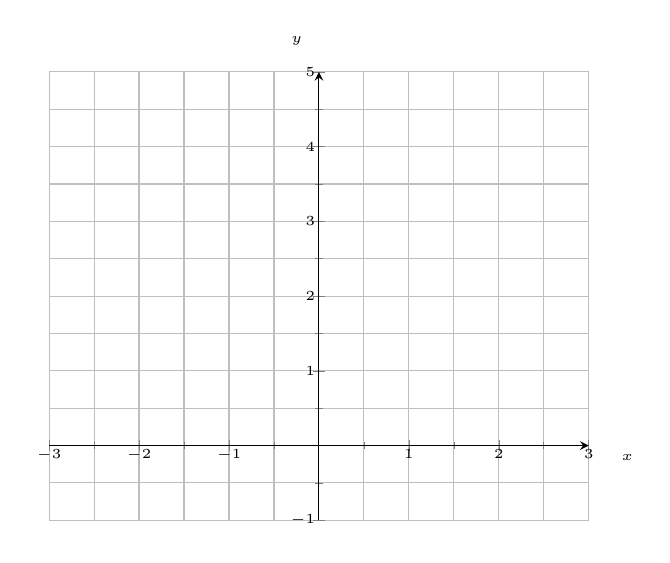
\begin{tikzpicture}
 \begin{axis}[grid=both, ymin=-1,ymax=5,xmax=3,xmin=-3,xtick={-3,-2,...,3},ytick={-1,0,...,5},minor tick num=1, axis lines = middle,xlabel=$x$,ylabel=$y$, 
x tick label style={yshift=1ex,font={\tiny}}, y tick label style={xshift=1ex, font={\tiny}}, label style ={at={(ticklabel cs:1.1)}, font={\tiny}}
]
 %\addplot[thick, samples=100,domain=1:3.82, name path=A, -stealth]   {(x-2)^2+1};           
 % \addplot[thick, draw] (1, 2)--(-1.95,1.5);
 % \node[draw,shape=circle, minimum size=1.25mm,inner sep=0pt,outer sep=0pt] at (-2,1.5) {};              
  \end{axis}
\end{tikzpicture}
\end{center}
\end{minipage}
\end{minipage}
\end{exercise}


